\documentclass[a4paper,11pt]{scrartcl}
\usepackage[T1]{fontenc}
\usepackage[utf8x]{inputenc}
\usepackage{graphicx}
\usepackage{xcolor}

% \usepackage{tgheros}
% \usepackage[defaultmono]{droidmono}

\usepackage{amsmath,amssymb,amsthm,textcomp}
\usepackage{enumerate}
\usepackage{multicol}
\usepackage{tikz}

\usepackage{menukeys}

\usepackage{geometry}
\geometry{total={210mm,297mm},
left=25mm,right=25mm,%
bindingoffset=0mm, top=20mm,bottom=30mm}

\linespread{1.2}

\newcommand{\linia}{\rule{\linewidth}{0.5pt}}

% my own titles
\makeatletter
\renewcommand{\maketitle}{
\begin{center}
\vspace{2ex}
{\huge \@title}
\vspace{1ex}
\\
\linia\\
\@author \hfill \@date
\vspace{4ex}
\end{center}
}
\makeatother
%%%

% custom footers and headers
\usepackage{fancyhdr}
\pagestyle{fancy}
\lhead{}
\chead{}
\rhead{}
\lfoot{\mytitle}
\cfoot{}
\rfoot{\thepage}
\renewcommand{\headrulewidth}{0pt}
\renewcommand{\footrulewidth}{0.5pt}

%

% code listing settings
\usepackage{listings}
\lstset{
    language=Python,
    basicstyle=\ttfamily\small,
    aboveskip={1.0\baselineskip},
    belowskip={1.0\baselineskip},
    columns=fixed,
    extendedchars=true,
    breaklines=true,
    tabsize=4,
    prebreak=\raisebox{0ex}[0ex][0ex]{\ensuremath{\hookleftarrow}},
    frame=lines,
    showtabs=false,
    showspaces=false,
    showstringspaces=false,
    keywordstyle=\color[rgb]{0.627,0.126,0.941},
    commentstyle=\color[rgb]{0.133,0.545,0.133},
    stringstyle=\color[rgb]{01,0,0},
    numbers=left,
    numberstyle=\small,
    stepnumber=1,
    numbersep=10pt,
    captionpos=t,
    escapeinside={\%*}{*)}
}

% Inline graphics
\usepackage{graphicx,calc}
\newlength\myheight
\newlength\mydepth
\settototalheight\myheight{Xygp}
\settodepth\mydepth{Xygp}
\setlength\fboxsep{0pt}
\newcommand*\inlinegraphics[1]{%
  \settototalheight\myheight{Xygp}%
  \settodepth\mydepth{Xygp}%
  \raisebox{-\mydepth}{\includegraphics[height=\myheight]{#1}}%
}

% Swift
\lstdefinelanguage{swift}
{
  morekeywords={
    func,if,then,else,for,in,while,do,switch,case,default,where,break,continue,fallthrough,return,
    typealias,struct,class,enum,protocol,var,func,let,get,set,willSet,didSet,inout,init,deinit,extension,
    subscript,prefix,operator,infix,postfix,precedence,associativity,left,right,none,convenience,dynamic,
    final,lazy,mutating,nonmutating,optional,override,required,static,unowned,safe,weak,internal,
    private,public,is,as,self,unsafe,dynamicType,true,false,nil,Type,Protocol,
  },
  morecomment=[l]{//}, % l is for line comment
  morecomment=[s]{/*}{*/}, % s is for start and end delimiter
  morestring=[b]" % defines that strings are enclosed in double quotes
}
\definecolor{keyword}{HTML}{BA2CA3}
\definecolor{string}{HTML}{D12F1B}
\definecolor{comment}{HTML}{008400}
\lstset{
  language=swift,
  basicstyle=\ttfamily,
  showstringspaces=false, % lets spaces in strings appear as real spaces
  columns=fixed,
  keepspaces=true,
  keywordstyle=\color{keyword},
  stringstyle=\color{string},
  commentstyle=\color{comment},
}
\lstset{language=Swift}

\begin{document}

\newcommand{\mytitle}{TP 3 - Unit Converter}
\title{\mytitle}
\author{Adrien Humilière}
\date{01/03/2017}

\maketitle

\section*{Part 1}

\begin{itemize}
\item Create a new project, of the kind \textbf{Single View Application}.
\item Using Interface Builder and the Object Library (\keys{\Alt+\cmd+L}), add a text label for the converted temperature.
\item Adjust the auto layout constraints of the label. It should be at a fixed distance of the top, and horizontally centered.
\item Using Interface Builder and the Object Library, add a Picker View to the bottom of the interface and adjust its constraints.
\item Run the app (\keys{\cmd+R}) and attempt to use the picker.
\end{itemize}

\section*{Part 2}

\begin{itemize}
\item The picker view allow the user to pick a text or a date within defined choices. It uses the data source and delegate patterns.
\item Using Interface Builder, set the main View Controller as the picker view datasource by Control-clicking on the picker view, and dragging a connection from the dataSource connection well to the View Controller in the Document Outline (\inlinegraphics{../assets/show-document-outline.png}).
\item Run the app, observe the crash, and inspect the console output.
\item The picker view's data source is the view controller, but the ViewController class does not yet implement the methods that conform to the \texttt{UIPickerViewDataSource} protocol.
\item Using the Xcode Documentation and API Reference (\keys{\shift+\cmd+0}), explore the \\\texttt{UIPickerViewDataSource} Protocol Reference and the methods \texttt{numberOfComponentsInPickerView:} and \texttt{pickerView:numberOfRowsInComponent:}.
\item Add the \texttt{UIPickerViewDataSource} protocol declaration to the controller class.
\begin{lstlisting}
class ViewController: UIViewController, UIPickerViewDataSource {
\end{lstlisting}
\item Open the Issue Navigator (\keys{\cmd+4}), and notice the warnings indicating the methods necessary for conforming to the \texttt{UIPickerViewDataSource} protocol.
\item Implement \texttt{numberOfComponentsInPickerView:} and \texttt{pickerView:numberOfRowsInComponent:}.
\begin{lstlisting}
func numberOfComponentsInPickerView(pickerView: UIPickerView) -> Int {
	return 1
}

func pickerView(pickerView: UIPickerView, numberOfRowsInComponent
	component: Int) -> Int {
	return 10
}
\end{lstlisting}
\item Run the app, and observe that the picker has one scrollable element that contains ten rows.
\end{itemize}

\section*{Part 3}

\begin{itemize}
\item Observe how the picker view displays the \texttt{?} character. Without a delegate to determine what to display, the picker view renders a \texttt{?} by default.
\item Using Interface Builder, set the main View Controller as the picker view delegate by Control-clicking the picker view, and dragging a connection from the delegate connection well to the View Controller in the Document Outline.
\item Add the \texttt{UIPickerViewDelegate} protocol declaration to the controller class.
\begin{lstlisting}
class ViewController: UIViewController, UIPickerViewDataSource, UIPickerViewDelegate {
\end{lstlisting}
\item Using the Xcode Documentation and API Reference, explore the \texttt{UIPickerViewDelegate} Protocol Reference and the methods \texttt{pickerView:titleForRow:forComponent:} and \\\texttt{pickerView:didSelectRow:inComponent:}.
\item In the \texttt{ViewController} class, implement \texttt{pickerView:titleForRow:forComponent:}.
\begin{lstlisting}
func pickerView(pickerView: UIPickerView, titleForRow row: Int, forComponent component: Int) -> String? {
	return "N Celsius degrees"
	}
\end{lstlisting}
\item In the \texttt{ViewController} class, implement \texttt{pickerView:didSelectRow:inComponent:}.
\begin{lstlisting}
func pickerView(pickerView: UIPickerView, didSelectRow row: Int, inComponent component: Int) {
	// convert and display temperature
	}
\end{lstlisting}
\item Add a custom breakpoint to \texttt{pickerView:didSelectRow:inComponent:} that generates a Log message containing \texttt{selected: @row@}.
\begin{figure}[h]
	\begin{center}
   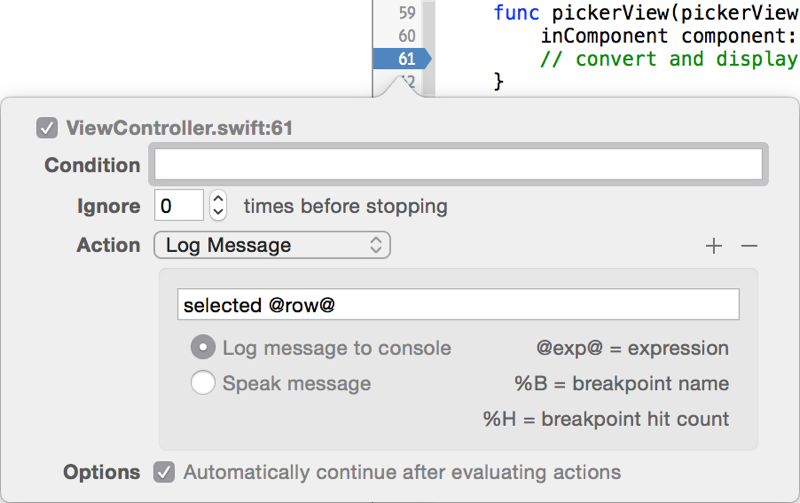
\includegraphics[width=200pt]{breakpoint.png}
	\end{center}
\end{figure}
\item Run the app, observe the values displayed in the picker view, flick the picker to select a row, and observe the console message when the row is selected.
\end{itemize}

\section*{Part 4}

\begin{itemize}
\item We want a "list" of negative and positive Celsius temperatures for the picker view to display, considering the total number of values (how many possible temperatures?), and the range (what minimum and maximum temperatures?).
\item In the controller, add a private property for an \texttt{Array} of temperature values that the controller will provide to the picker view for display.
\begin{lstlisting}
private var temperatureValues = [Int]()
\end{lstlisting}
\item Implement a naive, temporary assignment of the \texttt{temperatureValues} property during \texttt{viewDidLoad}.
\begin{lstlisting}
override func viewDidLoad() {
	super.viewDidLoad()
	temperatureValues = [1, 2, 3, 4, 5]
}
\end{lstlisting}
\item Update the implementation of \texttt{pickerView:titleForRow:forComponent:}.
\begin{lstlisting}
func pickerView(pickerView: UIPickerView, titleForRow row: Int, forComponent component: Int) -> String? {
	let celsiusValue = temperatureValues[row]
	return "\(celsiusValue) celsius degrees"
}
\end{lstlisting}
\item Run the app, observe the values displayed in the picker, and flick the picker one row at a time until the app crashes. Observe the console error.
\item Update \texttt{pickerView:titleForRow:forComponent:} to use the size of the \texttt{temperatureValues} array to inform the picker of how many rows to display.
\item Run the app, observe the temperature values, and interact with the picker.
\item Instead of an explicit array initialization([-100, -99, …, 99, 100]), a programmatic initialization using a loop will be used. Modify \texttt{viewDidLoad} to naively populate the temperatureValues array with a loop.
\begin{lstlisting}
override func viewDidLoad() {
	super.viewDidLoad()
	let lowerBound = -100
	let upperBound = 100
	for index in lowerBound...upperBound {
		temperatureValues.append(index)
	}
}
\end{lstlisting}
\item \texttt{map} might be used to transform a range into an array of \texttt{Int} values.
\item Using the documentation of \texttt{map}, update the \texttt{temperatureValues} property declaration and remove the procedural temperature value generation from \texttt{viewDidLoad}.
\item Run the app, and observe the temperature values in the picker.
\end{itemize}

\section*{Part 5}

\begin{itemize}
\item We now want to convert and display the temperature when selected in the picker view.
\item Using Interface Builder and the Assistant Editor (\keys{\Alt+\cmd+\return}), create an outlet connection for the label as a controller property.
\begin{lstlisting}
@IBOutlet weak var temperatureLabel: UILabel!
\end{lstlisting}
\item Update the ViewController \texttt{pickerView:didSelectRow:inComponent:} method. It will perform the conversion $farenheit=1.8\times celsius+32$ and update \texttt{temperatureLabel} with the value.
\item Run the app, select a temperature with the picker, and observe the displayed temperature.
\item We need to convert the converted temperature to an \texttt{Int} before updating the \texttt{UILabel} text property.
\end{itemize}

\section*{Part 6}

\begin{itemize}
\item The design pattern MVC (Model – View – Controller) is widely used in iOS development. It helps separating code logic from display. In this project, we will try to create a model taking care of the temperature conversion, to extract this logic from the view controller.
\item Add a new Swift class to the project for a UnitConverter model.
\begin{lstlisting}
import Foundation

class UnitConverter {

}
\end{lstlisting}
\item The temperature conversion code in the controller \texttt{pickerView:didSelectRow:inComponent:} method belongs in the model. Add a \texttt{degreesFahrenheit:} method to the \texttt{UnitConverter} class. It should take Celsius degrees in arguments (integers) and return Fahrenheit degrees (integers).
\item In the \texttt{ViewController} class, declare a new private property for a \texttt{UnitConverter} object and affect \texttt{UnitConverter()}.
\item Update the \texttt{pickerView:didSelectRow:inComponent:} method to use the \texttt{UnitConverter degreesFahrenheit:} method.
\end{itemize}

\section*{Part 7}

\begin{itemize}
\item The range of temperature values has nothing to do with unit conversion, and therefore the UnitConverter model should not be responsible of generating a range of temperatures. We will create a "view model": a model object whose sole purpose is to serve the view.
\item Add a new Swift class to the project for a \texttt{TemperatureRange} model.
\item We will now establish a \texttt{TemperatureRange} object as the picker view's \texttt{dataSource}. \texttt{TemperatureRange} will have to adopt the \texttt{UIPickerViewDataSource} protocol, and the picker view's \texttt{dataSource} connection will have to change to a new TemperatureRange object.
\item Using Interface Builder and the Object Library, drag an Object to the View Controller Scene in the Document Outline (\inlinegraphics{../assets/show-document-outline.png}). Rename the Object to \texttt{TemperatureRange}.
\begin{figure}[h]
	\begin{center}
   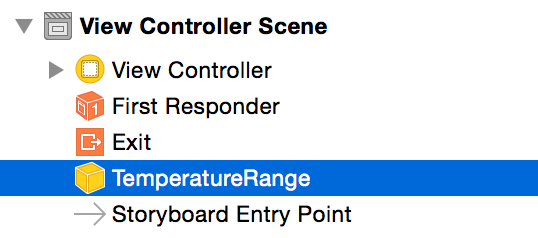
\includegraphics[width=100pt]{temperaturerange.png}
	\end{center}
\end{figure}
\item With the \texttt{TemperatureRange} object selected, use the Identity Inspector (\keys{\Alt+\cmd+3}) to set the Class to \texttt{TemperatureRange}.
\begin{figure}[h]
	\begin{center}
   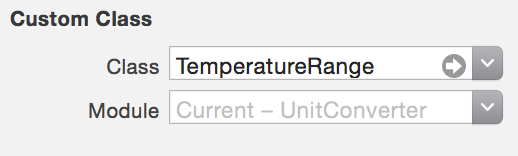
\includegraphics[width=100pt]{identityinspector.png}
	\end{center}
\end{figure}
\item Using Interface Builder, select the picker view and use the Connections Inspector (\keys{\Alt+\cmd+6}) to delete the \texttt{dataSource} connection between the picker view and the controller. Drag a new connection from the picker view's dataSource to the TemperatureRange object in the Document Outline.
\item Run the app, observe the crash, and inspect the error displayed in the console. \texttt{TemperatureRange} should implement \texttt{UIPickerViewDataSource}.
\end{itemize}

\section*{Part 8}

\begin{itemize}
\item Change the \texttt{TemperatureRange} class import statement to provide access to the \\\texttt{UIPickerViewDataSource} type.
\begin{lstlisting}
import UIKit
\end{lstlisting}
\item Update the \texttt{TemperatureRange} class to inherit from \texttt{NSObject} and to adopt the \\\texttt{UIPickerViewDataSource} protocol. Remove the \texttt{UIPickerViewDataSource} protocol adoption from the \texttt{ViewController} class definition.
\begin{lstlisting}
class TemperatureRange: NSObject, UIPickerViewDataSource
class ViewController: UIViewController, UIPickerViewDelegate
\end{lstlisting}
\item Move the \texttt{temperatureValues} property out of the controller and into the \texttt{TemperatureRange} class. Remove the private access control modifier, and shorten its name to \texttt{values}.
\begin{lstlisting}
let values = (-100...100).map { $0 }
\end{lstlisting}
\item Move the controller methods \texttt{numberOfComponentsInPickerView:} and \\\texttt{pickerView:numberOfRowsInComponent:} into the \texttt{TemperatureRange} class, and replace the reference to \texttt{temperatureValues} with \texttt{values}.
\begin{lstlisting}
func numberOfComponentsInPickerView(pickerView: UIPickerView) -> Int {
	return 1
}

func pickerView(pickerView: UIPickerView,
	numberOfRowsInComponent component: Int) -> Int {
	return values.count
}
\end{lstlisting}
\item Open the \texttt{ViewController} class, and observe the red error indicators.
\item Using Interface Builder and the Assistant Editor, Control-drag an outlet connection from the \texttt{TemperatureRange} object to the controller class, to create a new property.
\begin{lstlisting}
@IBOutlet var temperatureRange: TemperatureRange!
\end{lstlisting}
\item Update the controller methods \texttt{pickerView:titleForRow:forComponent:} and \\\texttt{pickerView:didSelectRow:inComponent:} to use the new \texttt{temperatureRange} property, replacing references to \texttt{temperatureValues} with \texttt{temperatureRange.values}.
\item Run the app, select a temperature, and observe the converted value.
\item The remaining controller code only manages communication between the view and the models, and updates the view.
\end{itemize}

\section*{Part 9}

\begin{itemize}
\item We want to improve the user experience when first starting the app. Notice the default starting temperature in the picker view, and consider how it affects the user experience. We might implement the behavior of specifying a default starting temperature.
\item Using Interface Builder and the Assistant Editor, add the picker view as an outlet property within the \texttt{ViewController} class.
\begin{lstlisting}
@IBOutlet weak var celsiusPicker: UIPickerView!
\end{lstlisting}
\item Set the default selected temperature in \texttt{viewDidLoad} with the method \\\texttt{selectRow:inComponent:animated:}.
\item Run the app and notice that, while the selected Celsius temperature has changed, the converted temperature label has not updated. Make sure the label is updated in \texttt{viewDidLoad}.
\item Run the app, observe the default selected temperature in the picker, and observe the converted temperature label.
\end{itemize}

\section*{Part 10}

\begin{itemize}
\item Run the app, select a temperature, background the app, then foreground the app. Notice how the last selected temperature is still displayed.
\item Using the multitasking bar (\keys{\shift+\cmd+H} twice quickly), quit the app, then start the app. The app "forgets" the last selected temperature, and displays the default temperature in the picker view. We want the app to "remember" the last selected temperature, and to use that temperature when it starts, if a last-selected temperature is known.
\item \texttt{NSUserDefaults} allow developers to save data in the filesystem as property list (.plist) files.
\item Enhance \texttt{pickerView:didSelectRow:inComponent:} to save the picker view's selected row index.
\begin{lstlisting}
let defaults = NSUserDefaults.standardUserDefaults()
defaults.setInteger(row, forKey: "defaultCelsiusPickerRow")
defaults.synchronize()
\end{lstlisting}
\item The controller method \texttt{pickerView:didSelectRow:inComponent:} now has two responsibilities: updating the temperature label and saving the last-selected row. Extract the code for each respective task into two separate, well-named controller methods.
\begin{lstlisting}
func displayConvertedTemperatureForRow(row: Int)
func saveSelectedRow(row: Int)
\end{lstlisting}
\item Update \texttt{pickerView:didSelectRow:inComponent:} to call the two new methods.
\item Extract the buried string into a constant placed near the top of the \texttt{ViewController} class. Use this constant in \texttt{saveSelectedRow:}.
\begin{lstlisting}
let userDefaultsLastRowKey = "defaultCelsiusPickerRow"
\end{lstlisting}
\item Run the app, select a temperature. Using the multitasking bar, quit the app, start the app again, and observe that, despite saving the last selected picker row, the default row is selected.
\end{itemize}

\section*{Part 11}

\begin{itemize}
\item Refactor \texttt{viewDidLoad} to use an \texttt{initialPickerRow} method, instead of a local variable, to determine the initial selected row index of the picker view.
\begin{lstlisting}
override func viewDidLoad() {
	super.viewDidLoad()
	let row = initialPickerRow()
	celsiusPicker.selectRow(row, inComponent: 0, animated: false)
	pickerView(celsiusPicker, didSelectRow: row, inComponent: 0)
}

func initialPickerRow() -> Int {
	// load from user defaults
	// if we obtained a last-known row index, return it
	// otherwise, return the default.
	return celsiusPicker.numberOfRowsInComponent(0) / 2
}
\end{lstlisting}
\item Using the Xcode documentation and API Reference, explore the \texttt{NSUserDefaults integerForKey:} method, and observe how it returns \texttt{0} when a value for the provided key is not found.
\item Implement a functional version of the \texttt{initialPickerRow} method, that fetch the corresponding data from \texttt{NSUserDefaults} and fallback to the default value if needed.
\item Run the app, select a temperature, force quit the app via the multitasking bar, restart the app, and witness the last selected temperature is correctly displayed.
\end{itemize}


\end{document}
